\documentclass[11pt]{article}
\usepackage[a4paper,margin=2.2cm]{geometry}
\usepackage{booktabs}
\usepackage{graphicx}
\usepackage{xcolor}
\usepackage{amsmath}
\usepackage{siunitx}
\usepackage{array}
\usepackage{caption}
\usepackage[colorlinks=true,linkcolor=blue!55!black,urlcolor=blue!55!black]{hyperref}
\usepackage{titlesec}

\definecolor{acc}{HTML}{2c5aa0}
\titleformat{\section}{\large\bfseries\color{acc}}{\thesection}{0.6em}{}
\titleformat{\subsection}{\normalsize\bfseries\color{acc!85!black}}{\thesubsection}{0.5em}{}
\captionsetup{font=small,labelfont={bf,color=acc}}
\newcommand{\uM}{\ensuremath{\mu}M}
\newcommand{\spn}[1]{\textit{#1}}
\setlength{\parskip}{4pt}
\setlength{\parindent}{0pt}
\renewcommand{\arraystretch}{1.15}

\begin{document}

\begin{center}
{\LARGE\bfseries AMPGen --- AMP Challenge Submission Report}\\[4pt]
{\large A two-stage generative pipeline for antimicrobial peptide design}\\[6pt]
{\normalsize NeurIPS 2026 Competition Track (szczurek-lab AMP Challenge) \quad$\cdot$\quad Report date: 2026-09-17}\\[2pt]
{\small Backbone: ESM2-35M (\texttt{facebook/esm2\_t12\_35M\_UR50D}) \quad$\cdot$\quad Compute: Modal, single H100}
\end{center}
\vspace{2pt}
\hrule
\vspace{6pt}

This report documents the AMPGen \emph{submission}: the deliverables, the data behind them, the
generator and predictor that produce and rank the library, and how our internal metrics map to the
challenge's scoring. It is the submission-facing companion to the AMPGen method paper
(\texttt{reports/AMPGen\_Report.pdf}), which carries the full training methodology and ablations.

\section{Submission summary}

AMPGen is a two-stage pipeline. \textbf{Stage-1} is an activity-blind generator (a domain-adapted
masked-language model over the full AMP corpus, used as a Gibbs mutation proposer) that produces
natural-like candidate peptides. \textbf{Stage-2} is a dual-endpoint predictor on the same frozen
encoder that scores each candidate for antibacterial activity (per-species MIC) and safety
(human-RBC HC50), and ranks the library. Deliverables:

\begin{itemize}\itemsep2pt
  \item A \textbf{50{,}000-sequence FASTA library} of designed peptides satisfying the challenge
        constraints (20 standard amino acids, length 8--50, linear, free termini).
  \item A \textbf{ranked top-100 list}, ordered by the predictor's activity/selectivity score, with
        every entry $\le 80\%$ identical to any DBAASP/dbAMP/APD reference (novelty gate).
  \item The generator and predictor weights, training data manifest, and this report.
\end{itemize}

\section{Challenge task and scoring metrics}

Submissions are scored by the organisers' \texttt{seqme} library against a fixed \textbf{20-strain
panel} (15 Gram-negative, 5 Gram-positive; an 8-strain MDR ESKAPE subset) across \textbf{five
categories}. The table gives what each category rewards and the underlying quantities.

\begin{table}[h]\centering\small
\caption{Challenge scoring categories and the quantities they reward. Potency threshold $=16$~\uM;
MIC ceiling $=64$~\uM; HC50 ceiling $=128$~\uM.}
\begin{tabular}{@{}p{3.1cm}p{7.2cm}p{5.2cm}@{}}
\toprule
\textbf{Category} & \textbf{What it rewards} & \textbf{Underlying quantity} \\
\midrule
Broad-Spectrum & Activity across the whole 20-strain panel & Success Rate over all strains \\
Gram-Positive & Activity on the 5 Gram+ strains & Success Rate / MIC50 (Gram+) \\
Gram-Negative & Activity on the 15 Gram$-$ strains & Success Rate / MIC50 (Gram$-$) \\
MDR ESKAPE & Activity on the 8-strain drug-resistant subset & Success Rate (MDR subset) \\
Optimal Selectivity & Potent \emph{and} non-toxic to human cells & Safety Window $=$ HC50 / MIC50 \\
\bottomrule
\end{tabular}
\end{table}

\textbf{Function of each scoring quantity.}
\begin{itemize}\itemsep1pt
  \item \textbf{Success Rate} --- fraction of panel strains for which a peptide reaches
        MIC $\le 16$~\uM\ (the potency threshold). The core ``does it work'' measure; drives the
        four activity categories.
  \item \textbf{MIC50 / MIC90} --- median / 90th-percentile MIC across the relevant strain set;
        summarise potency depth and breadth.
  \item \textbf{Safety Window (HC50/MIC50)} --- how much more concentrated a peptide must be to lyse
        human red blood cells than to kill bacteria; the therapeutic-index proxy that defines the
        Optimal-Selectivity category.
\end{itemize}

\section{Data sources and scale}

All three data assets are unions of curated public databases, de-duplicated and split leak-free
(CD-HIT at 80\% identity, whole clusters assigned to train or test so no test sequence is $>\!80\%$
identical to any training sequence).

\begin{table}[h]\centering\small
\caption{Data assets behind the submission. MIC and HC50 feed the two predictor endpoints; the
generator corpus is the Stage-1 pretraining set.}
\begin{tabular}{@{}p{2.4cm}p{6.8cm}rrp{2.4cm}@{}}
\toprule
\textbf{Asset} & \textbf{Sources (union)} & \textbf{Seqs} & \textbf{Meas.} & \textbf{Notes} \\
\midrule
Generator corpus & AMPSphere T1+T2 (physchem-matched) $+$ DRAMP $+$ DBAASP $+$ dbAMP $+$ APD &
155{,}280 & --- & all-AMP MLM pretrain \\
MIC (10 species) & GRAMPA $+$ ampbench-v0.7 master $+$ AMPBench-MT & 13{,}123 & 40{,}874 &
$\log_{10}$ \uM; 14 flags free-termini \\
HC50 (human RBC) & ampbench master \texttt{hc50\_human} (DBAASP+HemoPI2+Hemolytik+QMAP+DRAMP)
$+$ Hemolytik2 $+$ DRAMP text & 4{,}402 & 4{,}402 & 14.2\% right-censored \\
\bottomrule
\end{tabular}
\end{table}

\begin{table}[h]\centering\small
\caption{MIC measurement scale per panel species (post-union, 10 species). AMPBench-MT contributes
the DBAASP rare-species MIC our earlier GRAMPA$+$master build did not include, multiplying the
low-data species 3--13$\times$.}
\begin{tabular}{@{}lrrr@{}}
\toprule
\textbf{Species} & \textbf{Gram} & \textbf{measurements} & \textbf{panel strains} \\
\midrule
\spn{E. coli}        & $-$ & 11{,}143 & 5 \\
\spn{S. aureus}      & $+$ & 9{,}776  & 2 \\
\spn{P. aeruginosa}  & $-$ & 6{,}977  & 3 \\
\spn{B. subtilis}    & $+$ & 3{,}139  & 1 \\
\spn{S. enterica}    & $-$ & 2{,}393  & 2 \\
\spn{K. pneumoniae}  & $-$ & 2{,}353  & 2 \\
\spn{A. baumannii}   & $-$ & 2{,}025  & 2 \\
\spn{E. faecalis}    & $+$ & 1{,}779  & 1 \\
\spn{E. faecium}     & $+$ & 771      & 1 \\
\spn{E. cloacae}     & $-$ & 518      & 1 \\
\midrule
\textbf{Total}      &     & \textbf{40{,}874} & \textbf{20} \\
\bottomrule
\end{tabular}
\end{table}

\section{Stage-1 --- Generator}

The generator is a domain-adaptive masked-LM pretrain of ESM2-35M on the 155{,}280-sequence all-AMP
corpus (variable-rate span/scattered masking, $1/t$-reweighted cross-entropy, 3 epochs), used as a
temperature-sampled mutation proposer. It is judged on whether its output is \emph{natural-like} on
the axes that matter for AMPs (physicochemical marginals and an independent language-model
naturalness score), not on exact-residue recovery.

\begin{table}[h]\centering\small
\caption{Generator (Stage-1) held-out metrics. Reference = held-out natural AMPs; pseudo-perplexity
is from an independent ESM2-150M, distinct from the generator backbone.}
\begin{tabular}{@{}lrrl@{}}
\toprule
\textbf{Metric} & \textbf{init} & \textbf{final} & \textbf{reference / comparator} \\
\midrule
Validation loss                         & 2.633 & 2.236 & --- \\
Exact masked-token recovery             & 0.193 & 0.277 & chance 0.05 ($>3\times$) \\
Novelty, fraction $\le 80\%$ identity   & ---   & 100\% & challenge novelty gate \\
Embedding diversity (mean pairwise cos-dist) & --- & 0.0977 & natural 0.1009 (matched) \\
Pseudo-perplexity, median               & ---   & 17.12 & natural 17.01 (near-identical) \\
Wasserstein: len / charge / GRAVY / $\mu$H / hydrophobic & --- & \multicolumn{2}{l}{0.000 / 0.099 / 0.014 / 0.005 / 0.002 (lower $=$ closer)} \\
\bottomrule
\end{tabular}
\end{table}

The generator reproduces the natural AMP marginal (physchem Wasserstein near zero on every axis,
pseudo-perplexity matched to natural) and passes the novelty gate at 100\%, i.e. it neither collapses
to a degenerate mode nor drifts out-of-distribution.

\section{Stage-2 --- Dual-endpoint predictor}

On the frozen Stage-1 encoder we train LoRA (r=8, $\alpha$=16, last 4 attention layers; 0.79~M
trainable params, 2.3\%) feeding two heads: a \textbf{species-conditioned MIC head} (AdaLN over 10
species) predicting $-\log_{10}$MIC, and a \textbf{single HC50 head} predicting $\log_{10}$HC50.
Both are trained to \emph{absolute} $\log_{10}$~\uM\ with a composite loss (pairwise ranking $+$
Huber magnitude regression); the HC50 loss is censoring-aware (right-censored ``safe-tail''
measurements penalised one-sidedly). The two heads are trained as \textbf{separate} models
(shared frozen encoder, own LoRA) --- multitask training gave no MIC gain and a clear HC50 loss
(the small-task seesaw), so separate is the final configuration.

\subsection{Version progression (v1 $\to$ v3)}

\begin{table}[h]\centering\small
\caption{Predictor performance across iterations, overall Spearman $\rho$ / Pearson $r$ on the honest
(homology) split, plus the random-split $\rho$. v1 $=$ dual-endpoint baseline; v2 adds
rare-species sampling rebalance and censoring-aware HC50 loss; v3 adds the AMPBench-MT data merge.}
\begin{tabular}{@{}llcccc@{}}
\toprule
\textbf{Ver} & \textbf{Change} & \textbf{MIC $\rho$/$r$ (hon)} & \textbf{HC50 $\rho$/$r$ (hon)}
 & \textbf{MIC $\rho$ (rand)} & \textbf{HC50 $\rho$ (rand)} \\
\midrule
v1 & dual-endpoint baseline & 0.578 / 0.592 & 0.456 / 0.478 & 0.645 & 0.597 \\
v2 & $+$ rebalance $+$ censoring & \textbf{0.585 / 0.597} & \textbf{0.503 / 0.522} & 0.637 & 0.563 \\
v3 & $+$ AMPBench-MT data & 0.494 / 0.512$^{\dagger}$ & 0.421 / 0.459$^{\dagger}$ & 0.619 & 0.592 \\
\bottomrule
\end{tabular}
\end{table}

\begin{figure}[h]\centering
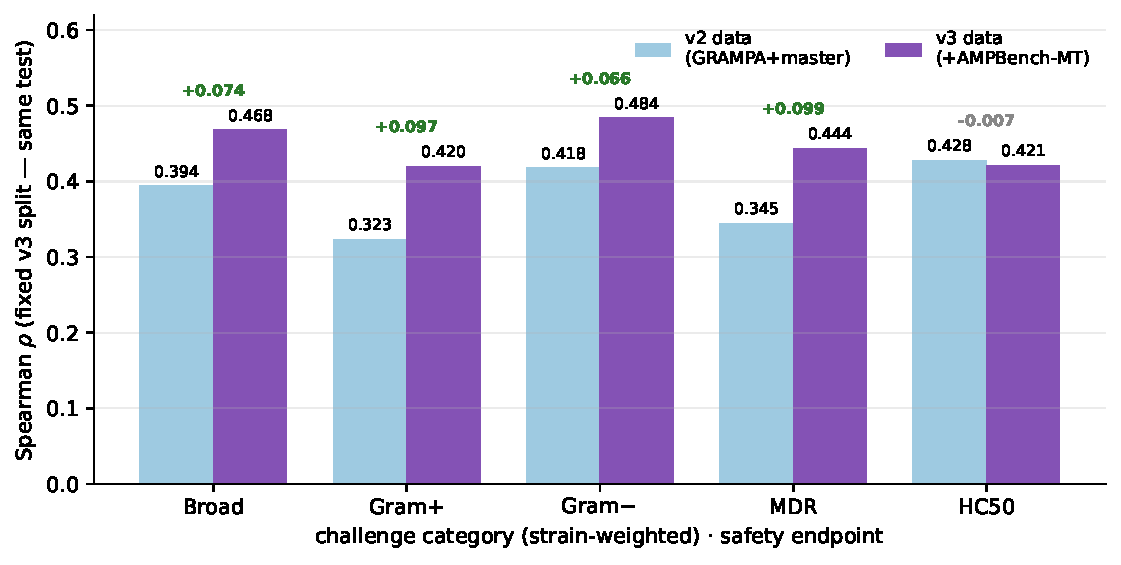
\includegraphics[width=0.86\textwidth]{figures/predictor_performance.pdf}
\caption{Predictor performance across versions v1--v3 (bar colour) on the honest homology split, at
the \emph{challenge-category} level: the four MIC categories are strain-count-weighted means of the
per-species Spearman $\rho$ (via the panel aggregation of \S\ref{sec:agg}), and HC50 is the safety
endpoint. v2 is best on every category; v3 dips because its re-clustered test set is harder
(see $\dagger$), not because the added data hurts.}
\end{figure}

$^{\dagger}$\,\textbf{v3 honest numbers are confounded by re-clustering.} Adding 16{,}821 MIC rows
changed the global CD-HIT clustering, so the v3 honest test set differs from v2's and is harder.
The proof: HC50's data is \emph{unchanged} between v2 and v3, yet its honest $\rho$ moved
$0.503\!\to\!0.421$ ($-0.082$) purely from the re-split. MIC's $-0.091$ is therefore almost entirely
the harder split, not a regression. Net: the data merge is $\rho$-neutral on the overall honest
split while tripling-to-13$\times$-ing rare-species coverage --- a coverage gain for the
MDR/Gram categories rather than a headline-$\rho$ gain. \textbf{v2 remains the recommended
configuration by honest overall $\rho$}; the v3 data is retained for its rare-species coverage.

\subsection{Per-species MIC (honest split)}

\begin{table}[h]\centering\small
\caption{MIC Spearman $\rho$ per panel species on the honest split for the recommended v2 model, with
the v3 test-set size showing the coverage growth from the AMPBench-MT merge. Low-$n$ species carry
wide confidence intervals.}
\begin{tabular}{@{}lrrr@{}}
\toprule
\textbf{Species} & \textbf{v2 $\rho$} & \textbf{v2 test-$n$} & \textbf{v3 test-$n$} \\
\midrule
\spn{E. coli}       & 0.598 & 937 & 1142 \\
\spn{S. aureus}     & 0.550 & 774 & 1036 \\
\spn{P. aeruginosa} & 0.631 & 620 & 641 \\
\spn{B. subtilis}   & 0.546 & 90  & 338 \\
\spn{S. enterica}   & 0.578 & 48  & 231 \\
\spn{K. pneumoniae} & 0.590 & 47  & 207 \\
\spn{E. faecalis}   & 0.255 & 39  & 165 \\
\spn{E. cloacae}    & 0.356 & 25  & 68  \\
\spn{E. faecium}    & 0.469 & 19  & 80  \\
\spn{A. baumannii}  & 0.681 & 13  & 157 \\
\bottomrule
\end{tabular}
\end{table}

\section{Our evaluation metrics and their function}

The predictor is scored with four complementary metrics, on two splits, against a mean-predictor
baseline --- so that a number can never be read as good without its honest reference.

\begin{itemize}\itemsep2pt
  \item \textbf{Spearman $\rho$} (ranking, calibration-free) --- how well the score \emph{orders}
        peptides by activity/safety. This is what the \textbf{top-100 ranking} deliverable depends on.
  \item \textbf{Pearson $r$} (magnitude, on absolute $\log_{10}$\uM) --- whether predicted values track
        true values in \emph{absolute} terms. Required because the challenge scores an absolute
        16~\uM\ potency threshold and the HC50/MIC50 safety window; a rank-only model cannot supply
        these. We measure $r$ on \emph{raw} values, not by inverting a ranking score. Because
        $\rho\!\approx\!r$ (not $\rho\!\approx\!2r$), the model genuinely calibrates magnitude.
  \item \textbf{RMSE / MAE} ($\log_{10}$\uM) --- absolute error, reported against the mean-predictor's
        RMSE (its ceiling when $\rho\!=\!r\!=\!0$).
  \item \textbf{Split.} The \emph{homology} split (CD-HIT-80\% whole-cluster) is the honest,
        deployment-relevant number; the \emph{random} by-sequence split leaks homologs across
        train/test and is the inflated, literature-comparable number. We always report both.
\end{itemize}

\section{Panel aggregation --- species to category scores}\label{sec:agg}

The predictor emits one MIC per species and one HC50; the challenge scores a 20-strain panel. The
aggregation (\texttt{challenge/metrics/aggregate.py}) broadcasts each species' predicted MIC to the
panel strains it represents (\texttt{PANEL\_STRAIN\_COUNTS}: \spn{E.\,coli}$\times$5,
\spn{P.\,aeruginosa}$\times$3, \dots) and computes, per category, \textbf{Success Rate} (fraction of
strains with MIC $\le 16$~\uM), \textbf{MIC50/MIC90} (strain-weighted percentiles), and, for
Optimal-Selectivity, \textbf{Safety Window} $=$ HC50\,/\,MIC50 --- all with the challenge ceilings
(MIC 64~\uM, HC50 128~\uM) applied. Categories: Broad (all 20 strains), Gram$+$ (5), Gram$-$ (15),
MDR (the 8-strain ESKAPE subset). The same category weighting yields the category-level ranking
$\rho$ shown in Figure~1 and Table~6, where v2 leads every category.

\begin{table}[h]\centering\small
\caption{Category-level ranking quality: strain-count-weighted mean of per-species MIC Spearman
$\rho$ per challenge category (honest homology split), plus the HC50 safety endpoint, for each
version. v2 is best on every category; v3's dip is the re-clustering artifact ($\dagger$ above).}
\begin{tabular}{@{}lccccc@{}}
\toprule
\textbf{Version} & \textbf{Broad} & \textbf{Gram$+$} & \textbf{Gram$-$} & \textbf{MDR} & \textbf{HC50} \\
\midrule
v1 & 0.545 & 0.467 & 0.570 & 0.515 & 0.456 \\
v2 & \textbf{0.565} & \textbf{0.474} & \textbf{0.596} & \textbf{0.547} & \textbf{0.503} \\
v3 & 0.468 & 0.420 & 0.484 & 0.444 & 0.421 \\
\bottomrule
\end{tabular}
\end{table}

\section{Decision and status}

\textbf{Final predictor:} v2 configuration (separate mode) --- honest MIC $\rho$ 0.585 / $r$ 0.597
(RMSE 0.65 $\log_{10}$\uM), honest HC50 $\rho$ 0.503 / $r$ 0.522 --- with the v3 AMPBench-MT data
retained for its 3--13$\times$ rare-species coverage (valuable for the MDR ESKAPE and Gram
categories). The censoring-aware HC50 loss was a clear win ($\rho$ $+0.047$); the rare-species
sampling rebalance and the data merge together lift the data-starved species that the challenge's
resistance-focused categories weigh most. A physicochemical-feature branch was diagnosed out
(incremental $r$ $+0.015$ MIC / $\sim\!0$ HC50 --- ESM2 already subsumes the descriptors).

\textbf{Remaining work toward submission:} the fixed-seed 50{,}000 generation run (constraints as a
generation gate), the top-100 selection under the novelty gate (ranked by the aggregated
selectivity score of \S\ref{sec:agg}), and a \texttt{seqme} scoring mirror for local validation.

\end{document}
